\usepackage{stmaryrd}%! Author = zero
%! Date = 29/07/2024

\documentclass[a4paper, 12pt]{article}

\usepackage[english,russian]{babel}
\usepackage[T2A]{fontenc}
\usepackage[utf8]{inputenc}
\usepackage{geometry}
\usepackage{enumitem}
\usepackage{setspace}
\usepackage{amssymb}
\usepackage{graphicx}
\usepackage{float}
\usepackage{wrapfig}
\geometry{top=5mm}
\renewcommand{\arraystretch}{1.2}
\linespread{1}

% Document
\begin{document}
    \begin{center}
        \textbf{Задачи №5 Решение задач}\\
    \end{center}

    \begin{center}
        \textbf{ЕГЭ}\\
    \end{center}

    \begin{spacing}{1.1}
        \begin{enumerate}
            \item На числовой прямой даны два промежутка: $P = [25; 50]$ и $Q = [32; 47]$.
            Укажите наибольшую возможную длину промежутка $A$, для которого выражение
            $((x \in P) \leftrightarrow (x \in Q)) \rightarrow \overline{(x \in A)}$
            тождественно истинно при любом значении переменной $x$.7763

            \item На числовой прямой даны два промежутка: $P = [5; 30]$ и $Q = [14; 23]$.
            Укажите наибольшую возможную длину промежутка $A$, для которого выражение
            $(\overline{(x \in A)} \rightarrow (x \in P)) \rightarrow ((x \in A) \rightarrow (x \in Q))$
            тождественно истинно при любом значении переменной $x$.9653

            \item На числовой прямой даны два промежутка: $P = [4; 15]$ и $Q = [12; 20]$.
            Укажите наименьшую возможную длину отрезка $A$, для которого выражение
            $((x \in P) \wedge (x \in Q)) \rightarrow (x \in A)$
            тождественно истинно при любом значении переменной $x$. 9699

            \item На числовой прямой даны три промежутка: $P = [10; 40]$, $Q = [5; 15]$ и $R = [35; 50]$.
            Укажите наименьшую возможную длину отрезка $A$, для которого выражение
            $((x \in A) \vee (x \in P)) \vee ((x \in Q) \rightarrow (x \in R))$
            тождественно истинно при любом значении переменной $x$. 34535

            \item На числовой прямой даны три отрезка: $P = [10; 15]$, $Q = [10; 20]$ и $R = [5; 15]$.
            Укажите наименьшую возможную длину промежутка $A$, для которого выражения
            \[(x \in Q) \rightarrow (x \in R)\]
            \[(x \in A) \rightarrow (x \in P)\]
            принимают равные значения при любом значении переменной $x$. 34537

            \item На числовой прямой даны два отрезка: $P = [30; 45]$ и $Q = [40; 55]$.
            Укажите наименьшую возможную длину промежутка $A$, для которого выражения
            \[ \overline{x \in A} \rightarrow \overline{x \in P} \]
            \[ (x \in Q) \rightarrow (x \in A) \]
            тождественно истинны при любом значении переменной $x$. 34538

        \end{enumerate}
    \end{spacing}

    \newpage
    \begin{center}
        \textbf{Открытая олимпиада школьников по информатике ИТМО}
    \end{center}

    \begin{center}
        \textbf{№1 Сплошные следования}
    \end{center}

    Известно, что логическое высказывание $x \rightarrow y$ является истинным, а логическое высказывание $y \leftrightarrow z$ является ложным.
    Выберите среди перечисленных ниже высказываний все те, для которых в этом случае можно однозначно определить их
    логическое значение (истинность или ложность).
    \begin{enumerate}
        \item $(x \rightarrow y) \leftrightarrow z$
        \item $((x \wedge \overline y) \leftrightarrow (y \wedge z)) \rightarrow (y \leftrightarrow z)$
        \item $(x \rightarrow y) \rightarrow (y \oplus z)$
        \item $(\overline{z \oplus y}) \rightarrow (y \rightarrow z)$
        \item $(\overline y \wedge z) \rightarrow (y \leftrightarrow \overline x)$
    \end{enumerate}

    \begin{center}
        \textbf{№2 Затухание}
    \end{center}

    Упростите логическое выражение или укажите его результат (при его однозначности). Результат упрощения может
    содержать только операции инверсии, конъюнкции и дизъюнкции.

    \begin{figure}[h]
        \centering
        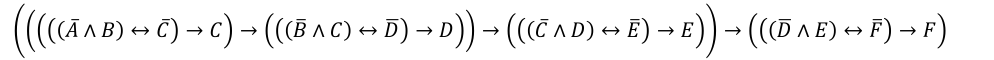
\includegraphics[width=1.2  \linewidth]{images/im1}
    \end{figure}

    Комментарий по вводу ответа: операнды вводятся большими латинскими буквами; логические операции обозначаются,
    соответственно как not, and и or.
    Скобки используются только для изменения порядка выполнения операций. Если порядок выполнения операций очевиден из
    их приоритетов – дополнительное использование скобок считается ошибкой.
    При однозначном ответе – истинный ответ обозначается как 1, а ложный как 0.
    Пример записи ответа: (A or not B) and C


    \begin{center}
        \textbf{№3 Полусумматоры}
    \end{center}

    Витя увлекается электротехникой и собирает различные логические схемы. На последнем занятии кружка электроники
    и электротехники руководитель кружка, Николай Александрович, рассказал про полусумматор.

    \textbf{Полусумматор} – это логическая схема, которая принимает на вход два логических значения $A$ и $B$ и выдаёт на выходе
    два логических значения $S$ и $C$ (сумму $A$ и $B$ с учётом переноса). Ниже представлена таблица истинности для такой схемы и
    пример её реализации с использованием исключающего ИЛИ и И:\\

    \begin{tabular}{|c|c|c|c|}
        \hline
        $A$ & $B$ & $S$ & $C$ \\
        \hline
        0   & 0   & 0   & 0   \\
        \hline
        0   & 1   & 1   & 0   \\
        \hline
        1   & 0   & 1   & 0   \\
        \hline
        1   & 1   & 0   & 1   \\
        \hline
    \end{tabular}

    \begin{figure}[h]
        \centering
        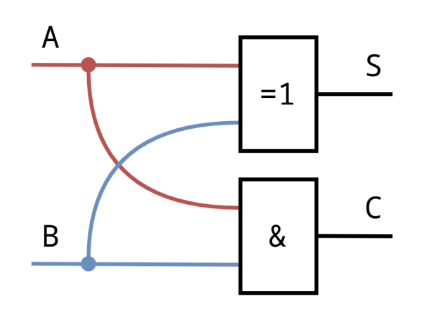
\includegraphics[width=0.3  \linewidth]{images/im2}
    \end{figure}

    Часто полусумматор обозначают на схемах как отдельный элемент.
    Оставшись после занятия, Витя решил собрать свою схему с использованием нескольких полусумматоров:

    \begin{figure}[h]
        \centering
        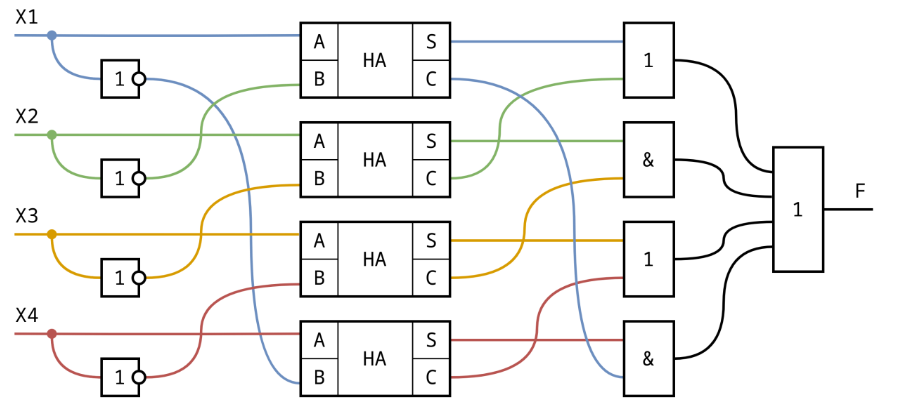
\includegraphics[width=1.0  \linewidth]{images/im3}
    \end{figure}
    Николай Александрович увидел схему и сказал, что эта схема будет выдавать ложь только для одной комбинации
    значений переменных. Найдите эту комбинацию и в ответе укажите подряд четыре значения $0$ или $1$, соответствующие
    значениям логических переменных в порядке возрастания их индексов, где $0$ означает ложное значение, а $1$ – истинное
    значение. Если таких комбинаций несколько, укажите любую из них. Если таких комбинаций нет, укажите в ответе $NULL$.
    Пример записи ответа: $1101$.

    Примечание: на схеме используются следующие обозначения логических элементов:
    \begin{figure}[h]
        \centering
        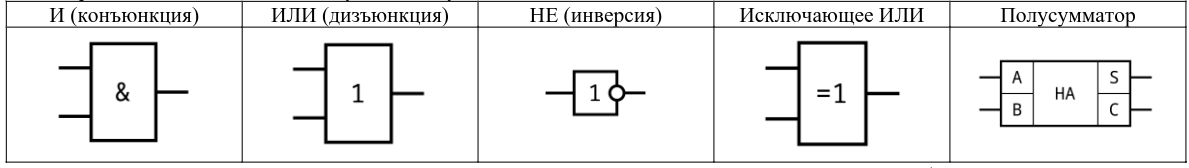
\includegraphics[width=1.1  \linewidth]{images/im4}
    \end{figure}

    Цвета на схеме предназначены для упрощения чтения и не несут никакой дополнительной информации.

\end{document}